\documentclass{standalone}
\usepackage{tikz}
\usetikzlibrary{patterns, positioning}


\begin{document}
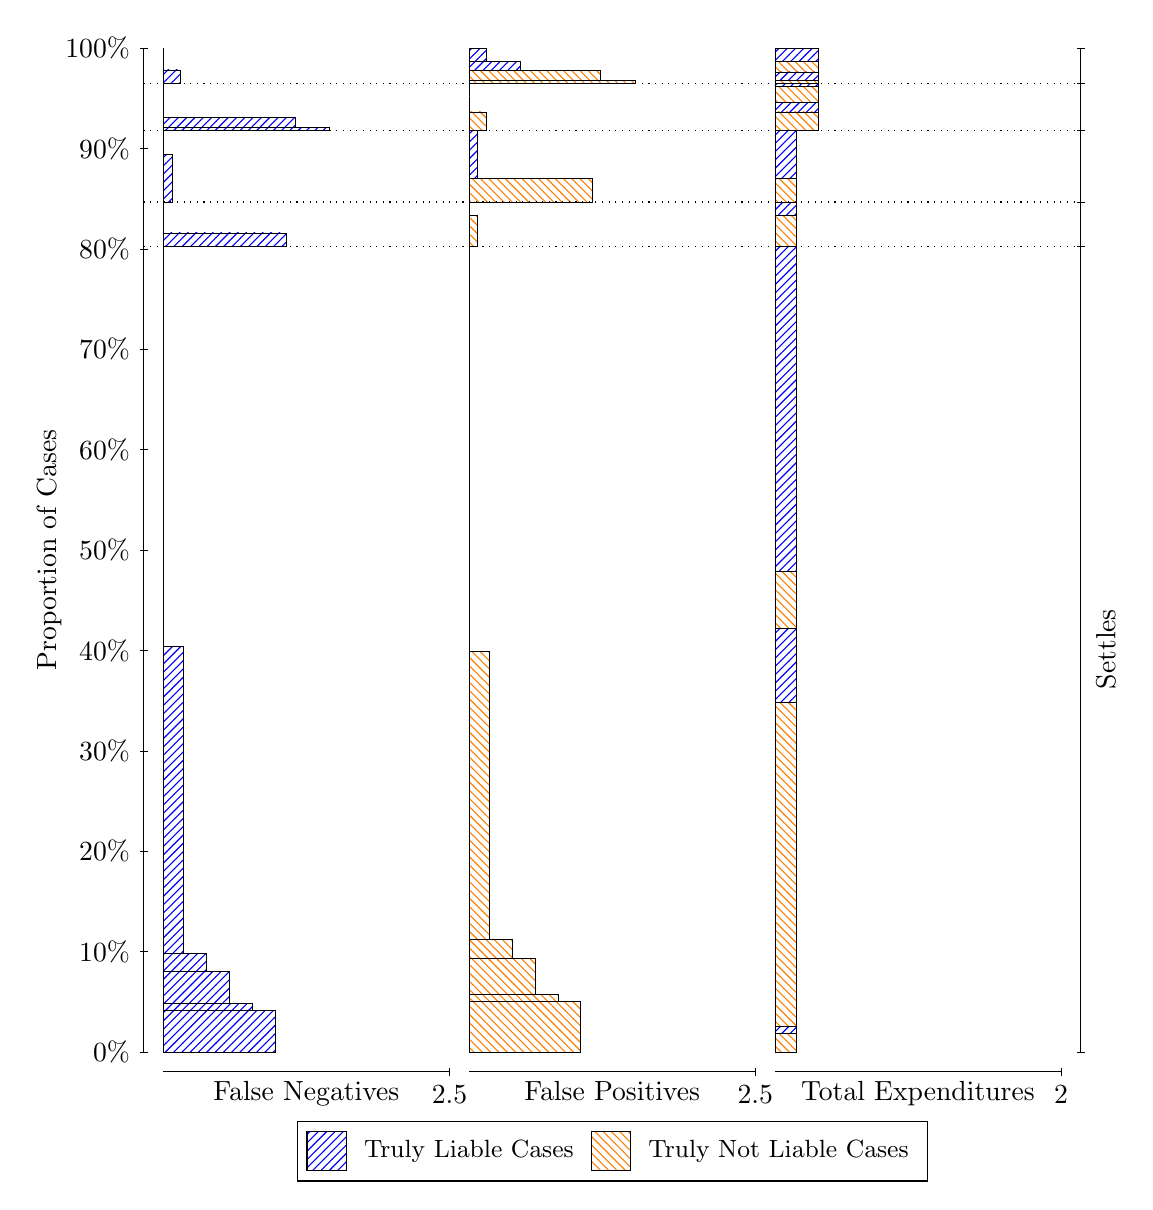
\begin{tikzpicture}
\draw[black, very thin] (1.5,1.75) -- (1.5,14.5);
\node[rotate=90, text=black, anchor=center] at (0.3, 8.125) {Proportion of Cases};
\draw[black, very thin] (1.45,1.75) -- (1.55,1.75);
\node[text=black, anchor=east] at (1.45, 1.75) {0\%};
\draw[black, very thin] (1.45,3.025) -- (1.55,3.025);
\node[text=black, anchor=east] at (1.45, 3.025) {10\%};
\draw[black, very thin] (1.45,4.3) -- (1.55,4.3);
\node[text=black, anchor=east] at (1.45, 4.3) {20\%};
\draw[black, very thin] (1.45,5.575) -- (1.55,5.575);
\node[text=black, anchor=east] at (1.45, 5.575) {30\%};
\draw[black, very thin] (1.45,6.85) -- (1.55,6.85);
\node[text=black, anchor=east] at (1.45, 6.85) {40\%};
\draw[black, very thin] (1.45,8.125) -- (1.55,8.125);
\node[text=black, anchor=east] at (1.45, 8.125) {50\%};
\draw[black, very thin] (1.45,9.4) -- (1.55,9.4);
\node[text=black, anchor=east] at (1.45, 9.4) {60\%};
\draw[black, very thin] (1.45,10.675) -- (1.55,10.675);
\node[text=black, anchor=east] at (1.45, 10.675) {70\%};
\draw[black, very thin] (1.45,11.95) -- (1.55,11.95);
\node[text=black, anchor=east] at (1.45, 11.95) {80\%};
\draw[black, very thin] (1.45,13.225) -- (1.55,13.225);
\node[text=black, anchor=east] at (1.45, 13.225) {90\%};
\draw[black, very thin] (1.45,14.5) -- (1.55,14.5);
\node[text=black, anchor=east] at (1.45, 14.5) {100\%};

\draw[black, very thin] (13.4,1.75) -- (13.4,14.5);
\draw[black, very thin] (13.35,1.75) -- (13.45,1.75);
\node[anchor=west] at (13.35, 1.75) {};
\draw[black, very thin] (13.35,11.982) -- (13.45,11.982);
\node[anchor=west] at (13.35, 11.982) {};
\draw[black, very thin] (13.35,12.544) -- (13.45,12.544);
\node[anchor=west] at (13.35, 12.544) {};
\draw[black, very thin] (13.35,13.453) -- (13.45,13.453);
\node[anchor=west] at (13.35, 13.453) {};
\draw[black, very thin] (13.35,14.051) -- (13.45,14.051);
\node[anchor=west] at (13.35, 14.051) {};
\draw[black, very thin] (13.35,14.5) -- (13.45,14.5);
\node[anchor=west] at (13.35, 14.5) {};

\draw[black, very thin, pattern color=blue, pattern=north east lines] (1.75,1.75) rectangle (3.167,2.2811);
\draw[black, very thin, pattern color=blue, pattern=north east lines] (1.75,2.2811) rectangle (2.8763,2.3715);
\draw[black, very thin, pattern color=blue, pattern=north east lines] (1.75,2.3715) rectangle (2.5857,2.7723);
\draw[black, very thin, pattern color=blue, pattern=north east lines] (1.75,2.7723) rectangle (2.295,3.005);
\draw[black, very thin, pattern color=blue, pattern=north east lines] (1.75,3.005) rectangle (2.0043,6.8962);
\draw[black, very thin, pattern color=orange, pattern=north west lines] (1.75,6.8962) rectangle (1.75,11.982);
\draw[black, very thin, pattern color=blue, pattern=north east lines] (1.75,11.982) rectangle (3.3123,12.152);
\draw[black, very thin, pattern color=orange, pattern=north west lines] (1.75,12.152) rectangle (1.75,12.544);
\draw[black, very thin, pattern color=blue, pattern=north east lines] (1.75,12.544) rectangle (1.859,13.154);
\draw[black, very thin, pattern color=orange, pattern=north west lines] (1.75,13.154) rectangle (1.75,13.453);
\draw[black, very thin, pattern color=blue, pattern=north east lines] (1.75,13.453) rectangle (3.8573,13.496);
\draw[black, very thin, pattern color=blue, pattern=north east lines] (1.75,13.496) rectangle (3.4213,13.621);
\draw[black, very thin, pattern color=orange, pattern=north west lines] (1.75,13.621) rectangle (1.75,14.051);
\draw[black, very thin, pattern color=blue, pattern=north east lines] (1.75,14.051) rectangle (1.968,14.222);
\draw[black, very thin, pattern color=orange, pattern=north west lines] (1.75,14.222) rectangle (1.75,14.389);
\draw[black, very thin, pattern color=blue, pattern=north east lines] (1.75,14.389) rectangle (1.75,14.5);
\draw[black, very thin, pattern color=orange, pattern=north west lines] (5.6333,1.75) rectangle (7.0503,2.392);
\draw[black, very thin, pattern color=orange, pattern=north west lines] (5.6333,2.392) rectangle (6.7597,2.4823);
\draw[black, very thin, pattern color=orange, pattern=north west lines] (5.6333,2.4823) rectangle (6.469,2.9435);
\draw[black, very thin, pattern color=orange, pattern=north west lines] (5.6333,2.9435) rectangle (6.1783,3.1763);
\draw[black, very thin, pattern color=orange, pattern=north west lines] (5.6333,3.1763) rectangle (5.8877,6.836);
\draw[black, very thin, pattern color=blue, pattern=north east lines] (5.6333,6.836) rectangle (5.6333,11.982);
\draw[black, very thin, pattern color=orange, pattern=north west lines] (5.6333,11.982) rectangle (5.7423,12.375);
\draw[black, very thin, pattern color=blue, pattern=north east lines] (5.6333,12.375) rectangle (5.6333,12.544);
\draw[black, very thin, pattern color=orange, pattern=north west lines] (5.6333,12.544) rectangle (7.1957,12.844);
\draw[black, very thin, pattern color=blue, pattern=north east lines] (5.6333,12.844) rectangle (5.7423,13.453);
\draw[black, very thin, pattern color=orange, pattern=north west lines] (5.6333,13.453) rectangle (5.8513,13.689);
\draw[black, very thin, pattern color=orange, pattern=north west lines] (5.6333,13.689) rectangle (5.6333,13.884);
\draw[black, very thin, pattern color=blue, pattern=north east lines] (5.6333,13.884) rectangle (5.6333,14.051);
\draw[black, very thin, pattern color=orange, pattern=north west lines] (5.6333,14.051) rectangle (7.7407,14.086);
\draw[black, very thin, pattern color=orange, pattern=north west lines] (5.6333,14.086) rectangle (7.3047,14.218);
\draw[black, very thin, pattern color=blue, pattern=north east lines] (5.6333,14.218) rectangle (6.2873,14.329);
\draw[black, very thin, pattern color=blue, pattern=north east lines] (5.6333,14.329) rectangle (5.8513,14.5);
\draw[black, very thin, pattern color=orange, pattern=north west lines] (9.5167,1.75) rectangle (9.7892,1.9828);
\draw[black, very thin, pattern color=blue, pattern=north east lines] (9.5167,1.9828) rectangle (9.7892,2.0732);
\draw[black, very thin, pattern color=orange, pattern=north west lines] (9.5167,2.0732) rectangle (9.7892,6.1941);
\draw[black, very thin, pattern color=blue, pattern=north east lines] (9.5167,6.1941) rectangle (9.7892,7.126);
\draw[black, very thin, pattern color=orange, pattern=north west lines] (9.5167,7.126) rectangle (9.7892,7.8583);
\draw[black, very thin, pattern color=blue, pattern=north east lines] (9.5167,7.8583) rectangle (9.7892,11.982);
\draw[black, very thin, pattern color=orange, pattern=north west lines] (9.5167,11.982) rectangle (9.7892,12.375);
\draw[black, very thin, pattern color=blue, pattern=north east lines] (9.5167,12.375) rectangle (9.7892,12.544);
\draw[black, very thin, pattern color=orange, pattern=north west lines] (9.5167,12.544) rectangle (9.7892,12.844);
\draw[black, very thin, pattern color=blue, pattern=north east lines] (9.5167,12.844) rectangle (9.7892,13.453);
\draw[black, very thin, pattern color=orange, pattern=north west lines] (9.5167,13.453) rectangle (10.062,13.689);
\draw[black, very thin, pattern color=blue, pattern=north east lines] (9.5167,13.689) rectangle (10.062,13.814);
\draw[black, very thin, pattern color=orange, pattern=north west lines] (9.5167,13.814) rectangle (10.062,14.008);
\draw[black, very thin, pattern color=blue, pattern=north east lines] (9.5167,14.008) rectangle (10.062,14.051);
\draw[black, very thin, pattern color=orange, pattern=north west lines] (9.5167,14.051) rectangle (10.062,14.086);
\draw[black, very thin, pattern color=blue, pattern=north east lines] (9.5167,14.086) rectangle (10.062,14.197);
\draw[black, very thin, pattern color=orange, pattern=north west lines] (9.5167,14.197) rectangle (10.062,14.329);
\draw[black, very thin, pattern color=blue, pattern=north east lines] (9.5167,14.329) rectangle (10.062,14.5);
\draw[black, dotted] (1.5,11.982) -- (13.4,11.982);
\draw[black, dotted] (1.5,12.544) -- (13.4,12.544);
\draw[black, dotted] (1.5,13.453) -- (13.4,13.453);
\draw[black, dotted] (1.5,14.051) -- (13.4,14.051);
\draw[black, very thin] (1.75,1.5) -- (5.3833,1.5);
\node[text=black, anchor=north] at (3.5667, 1.5) {False Negatives};
\draw[black, very thin] (5.3833,1.45) -- (5.3833,1.55);
\node[text=black, anchor=north] at (5.3833, 1.45) {2.5};

\draw[black, very thin] (5.6333,1.5) -- (9.2667,1.5);
\node[text=black, anchor=north] at (7.45, 1.5) {False Positives};
\draw[black, very thin] (9.2667,1.45) -- (9.2667,1.55);
\node[text=black, anchor=north] at (9.2667, 1.45) {2.5};

\draw[black, very thin] (9.5167,1.5) -- (13.15,1.5);
\node[text=black, anchor=north] at (11.333, 1.5) {Total Expenditures};
\draw[black, very thin] (13.15,1.45) -- (13.15,1.55);
\node[text=black, anchor=north] at (13.15, 1.45) {2};

\node[text=black, centered, rotate=90] at (13.72, 6.8661) {Settles};





\draw (7.449999999999999,1.5) node[draw=none] (baseCoordinate) {};
\begin{scope}[align=center]
        \matrix[scale=0.5, draw=black, below=0.5cm of baseCoordinate, nodes={draw}, column sep=0.1cm]{
            \node[rectangle, draw, minimum width=0.5cm, minimum height=0.5cm, pattern color=blue, pattern=north east lines] {}; &
            \node[draw=none, font=\small, text=black] (B) {Truly Liable Cases}; &
            \node[rectangle, draw, minimum width=0.5cm, minimum height=0.5cm, pattern color=orange, pattern=north west lines] {}; &
            \node[draw=none, font=\small, text=black] (B) {Truly Not Liable Cases}; \\
            };
\end{scope}

\end{tikzpicture}
\end{document}